\begin{tikzpicture}[x=1cm, y=1cm, font=\sffamily\footnotesize,
  ptitle/.style={anchor=west, font=\sffamily\bfseries\small, text=narrareddeep},
  textbox/.style={draw=phaseA!60, fill=phaseA!6, rounded corners=2pt, inner sep=4pt, anchor=north west,
                  align=left, font=\sffamily\scriptsize},
  lbl/.style={draw=#1, fill=white, fill opacity=0.9, text opacity=1, rounded corners=1pt, inner sep=1.6pt,
              line width=0.6pt, font=\sffamily\scriptsize},
  lblkey/.style={draw=#1, fill=white, fill opacity=0.95, text opacity=1, rounded corners=1pt, inner sep=1.8pt,
                 line width=1.0pt, font=\sffamily\scriptsize\bfseries},
  lead/.style={draw=#1, line width=0.7pt},
  path/.style={-{Latex[length=2.6mm, width=2.4mm]}, draw=black!85, line width=1.6pt},
  imgcap/.style={anchor=north, font=\sffamily\scriptsize, text=black!60},
  chip/.style={draw=black!30, fill=white, rounded corners=6pt, inner sep=2.5pt, font=\sffamily\footnotesize},
  flow/.style={-{Latex[length=1.6mm]}, draw=black!50, line width=0.6pt},
  lab/.style={anchor=east, font=\sffamily\footnotesize, text=black!75},
  txt/.style={anchor=west, font=\sffamily\footnotesize, text=black!75}]

\node[ptitle] at (0,0.000) {(a) The task and its room (AI2-THOR rendering of the benchmark trial)};
\node[textbox, text width=14.70cm] (obs) at (0,-0.280) {\textbf{Goal.} Your task is to: heat some egg and put it in garbagecan.\\[1pt]\textbf{Initial observation.} You are in the middle of a room. Looking quickly around you, you see a cabinet 6, a cabinet 5, a cabinet 4, a cabinet 3, a cabinet 2, a cabinet 1, a coffeemachine 1, a countertop 3, a countertop 2, a countertop 1, a drawer 3, a drawer 2, a drawer 1, a fridge 1, a garbagecan 1, a microwave 1, a shelf 3, a shelf 2, a shelf 1, a sinkbasin 1, a stoveburner 4, a stoveburner 3, a stoveburner 2, a stoveburner 1, and a toaster 1.};
\begin{scope}[shift={($(obs.south west)+(0,-0.25)$)}]
\node[anchor=north west, inner sep=0] at (0.000,0.000) {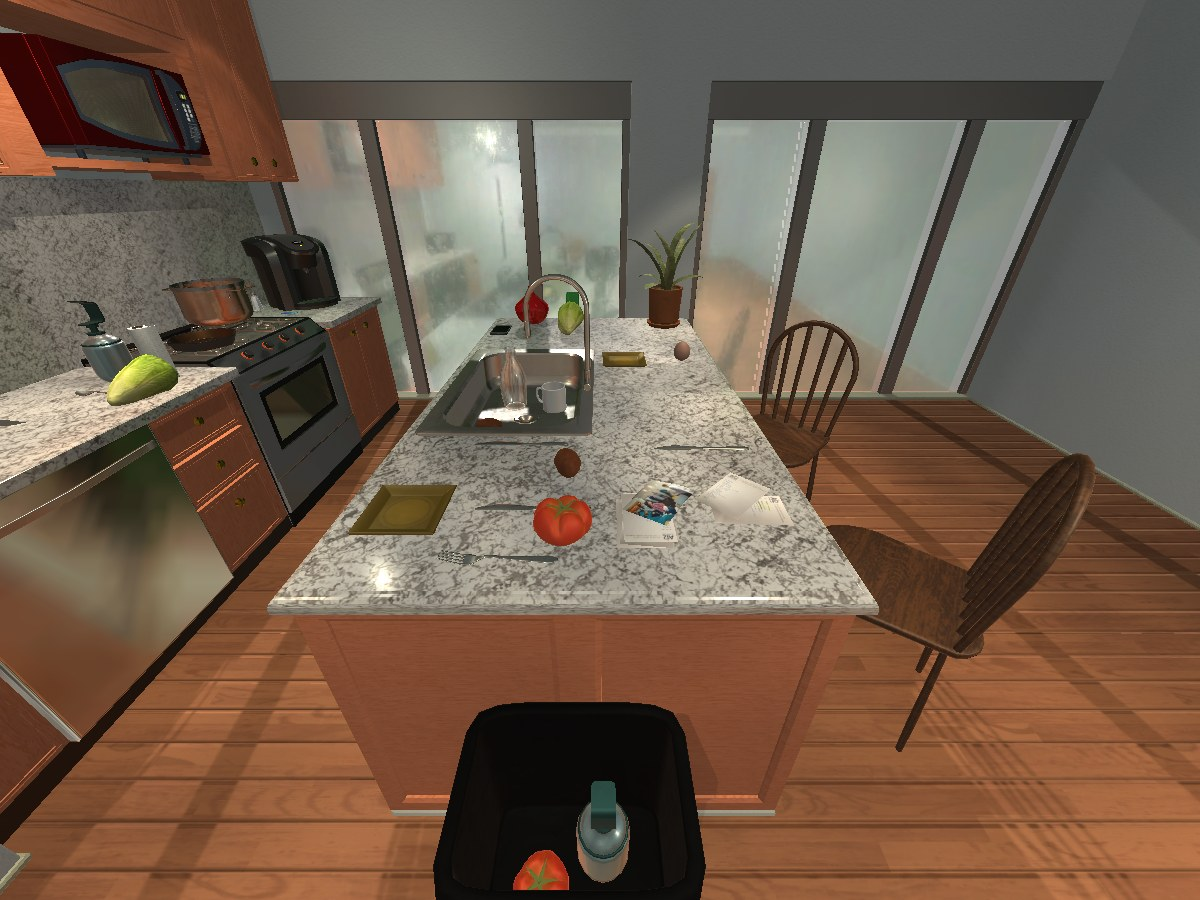
\includegraphics[width=8.815cm]{figures/cases/task1_view1.jpg}};
\draw[black!35, line width=0.4pt] (0.000,0.000) rectangle ++(8.815,-6.611);
\draw[dimF, line width=1.1pt] (5.006,-2.582) circle (0.160);
\draw[lead=dimF] (5.006,-2.582) -- (5.006,-2.082);
\fill[dimF] (5.006,-2.582) circle (0.06);
\node[lblkey=dimF] at (5.006,-2.082) {egg};
\draw[liftpositive, line width=1.1pt, rounded corners=1pt] (3.181,-5.164) rectangle (5.179,-6.611);
\draw[lead=liftpositive] (4.180,-5.888) -- (4.180,-5.388);
\fill[liftpositive] (4.180,-5.888) circle (0.06);
\node[lblkey=liftpositive] at (4.180,-5.388) {garbagecan: put it here};
\draw[dimA, line width=1.1pt, rounded corners=1pt] (2.101,-2.343) rectangle (6.325,-4.334);
\fill[dimA] (4.213,-3.339) circle (0.06);
\node[lblkey=dimA] at (4.213,-3.339) {countertop: the egg is here};
\draw[dimE, line width=1.1pt, rounded corners=1pt] (0.000,-0.250) rectangle (1.535,-1.212);
\draw[lead=dimE] (0.768,-0.731) -- (1.850,-1.084);
\fill[dimE] (0.768,-0.731) circle (0.06);
\node[lblkey=dimE] at (1.850,-1.084) {microwave: heat it here};
\draw[lead=black!55] (0.859,-3.122) -- (0.859,-2.622);
\fill[black!55] (0.859,-3.122) circle (0.06);
\node[lbl=black!45] at (0.859,-2.622) {countertops};
\draw[lead=black!55] (1.723,-0.668) -- (1.083,-0.315);
\fill[black!55] (1.723,-0.668) circle (0.06);
\node[lbl=black!45] at (1.083,-0.315) {cabinets};
\draw[lead=black!55] (1.763,-3.809) -- (1.763,-3.309);
\fill[black!55] (1.763,-3.809) circle (0.06);
\node[lbl=black!45] at (1.763,-3.309) {drawers};
\draw[lead=black!55] (2.130,-2.005) -- (2.130,-1.505);
\fill[black!55] (2.130,-2.005) circle (0.06);
\node[lbl=black!45] at (2.130,-1.505) {coffeemachine};
\node[anchor=north west, inner sep=0] at (9.065,0.000) {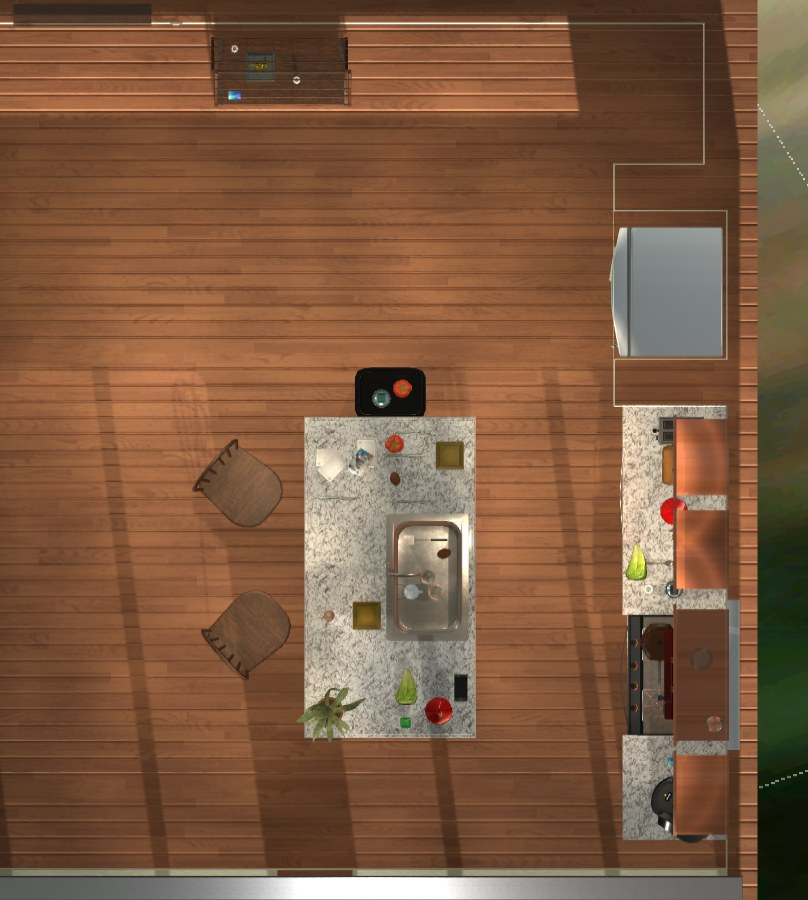
\includegraphics[width=5.935cm]{figures/cases/task1_map.jpg}};
\draw[black!35, line width=0.4pt] (9.065,0.000) rectangle ++(5.935,-6.611);
\fill[black, opacity=0.22] (11.874,-2.424) -- ++(-135:1.1) arc (-135:-45:1.1) -- cycle;
\fill[black] (11.874,-2.424) circle (0.08);
\draw[white, line width=3.4pt, opacity=0.85] (11.804,-4.290) -- (13.885,-4.885);
\draw[path] (11.804,-4.290) -- (13.885,-4.885);
\draw[white, line width=3.4pt, opacity=0.85] (13.979,-4.817) -- (12.115,-3.063);
\draw[path] (13.979,-4.817) -- (12.115,-3.063);
\draw[lead=dimA] (11.611,-4.235) -- (11.611,-3.735);
\fill[dimA] (11.611,-4.235) circle (0.06);
\node[lblkey=dimA] at (11.611,-3.735) {countertop: the egg is here};
\draw[lead=dimE] (14.125,-4.954) -- (13.043,-4.600);
\fill[dimE] (14.125,-4.954) circle (0.06);
\node[lblkey=dimE] at (13.043,-4.600) {microwave: heat it here};
\draw[lead=liftpositive] (11.933,-2.891) -- (10.851,-3.245);
\fill[liftpositive] (11.933,-2.891) circle (0.06);
\node[lblkey=liftpositive] at (10.851,-3.245) {garbagecan: put it here};
\draw[lead=black!55] (13.912,-3.766) -- (13.912,-3.266);
\fill[black!55] (13.912,-3.766) circle (0.06);
\node[lbl=black!45] at (13.912,-3.266) {cabinets};
\draw[lead=black!55] (13.912,-5.682) -- (13.912,-5.182);
\fill[black!55] (13.912,-5.682) circle (0.06);
\node[lbl=black!45] at (13.912,-5.182) {cabinets};
\draw[lead=black!55] (14.098,-5.925) -- (12.896,-5.734);
\fill[black!55] (14.098,-5.925) circle (0.06);
\node[lbl=black!45] at (12.896,-5.734) {coffeemachine};
\draw[lead=black!55] (14.003,-3.755) -- (14.003,-2.655);
\fill[black!55] (14.003,-3.755) circle (0.06);
\node[lbl=black!45] at (14.003,-2.655) {countertop};
\draw[lead=black!55] (14.003,-5.786) -- (13.305,-6.140);
\fill[black!55] (14.003,-5.786) circle (0.06);
\node[lbl=black!45] at (13.305,-6.140) {countertop};
\draw[lead=black!55] (13.679,-4.242) -- (14.289,-3.889);
\fill[black!55] (13.679,-4.242) circle (0.06);
\node[lbl=black!45] at (14.289,-3.889) {drawers};
\draw[lead=black!55] (14.041,-2.144) -- (14.041,-1.644);
\fill[black!55] (14.041,-2.144) circle (0.06);
\node[lbl=black!45] at (14.041,-1.644) {fridge};
\draw[lead=black!55] (11.115,-0.530) -- (10.215,-0.339);
\fill[black!55] (11.115,-0.530) circle (0.06);
\node[lbl=black!45] at (10.215,-0.339) {shelves};
\draw[lead=black!55] (12.207,-4.239) -- (10.776,-4.239);
\fill[black!55] (12.207,-4.239) circle (0.06);
\node[lbl=black!45] at (10.776,-4.239) {sinkbasin};
\draw[lead=black!55] (14.034,-4.960) -- (12.852,-4.182);
\fill[black!55] (14.034,-4.960) circle (0.06);
\node[lbl=black!45] at (12.852,-4.182) {stoveburners};
\draw[lead=black!55] (14.060,-3.164) -- (14.060,-2.064);
\fill[black!55] (14.060,-3.164) circle (0.06);
\node[lbl=black!45] at (14.060,-2.064) {toaster};
\node[imgcap] at (4.407,-6.651) {first-person view inside the room};
\node[imgcap] at (12.032,-6.651) {the room from above; cone: the left view; arrow: the expert's route};
\node[anchor=west, font=\sffamily\bfseries\footnotesize, text=black!70] at (0,-7.411) {Expert solution (6 steps):};
\node[chip, anchor=west] (s0) at (3.900,-7.411) {go to countertop};
\node[chip, anchor=west] (s1) at (6.872,-7.411) {take egg from countertop};
\draw[flow] (s0.east) -- (s1.west);
\node[chip, anchor=west] (s2) at (10.980,-7.411) {go to microwave};
\draw[flow] (s1.east) -- (s2.west);
\node[chip, anchor=west] (s3) at (3.900,-7.911) {heat egg with microwave};
\node[chip, anchor=west] (s4) at (7.866,-7.911) {go to garbagecan};
\draw[flow] (s3.east) -- (s4.west);
\node[chip, anchor=west] (s5) at (10.838,-7.911) {move egg to garbagecan};
\draw[flow] (s4.east) -- (s5.west);
\node[ptitle] at (0.000,-8.711) {(b) What happened: \texttt{GPT-4o-mini}, seed 0};
\node[lab] at (1.650,-9.311) {expert};
\fill[black!30, rounded corners=1pt] (1.750,-9.161) rectangle ++(1.200,-0.3);
\node[txt] at (3.030,-9.311) {6};
\node[lab] at (1.650,-9.771) {no memory};
\fill[phaseA!35, rounded corners=1pt] (1.750,-9.621) rectangle ++(6.000,-0.3);
\node[txt] at (7.830,-9.771) {30, not solved};
\node[lab] at (1.650,-10.231) {memory};
\fill[salmon!60, rounded corners=1pt] (1.750,-10.081) rectangle ++(6.000,-0.3);
\node[txt] at (7.830,-10.231) {30, not solved};
\draw[densely dashed, black!40] (7.750,-9.061) -- (7.750,-10.491);
\node[font=\sffamily\scriptsize, text=black!50, anchor=north] at (7.750,-10.491) {30-step limit};
\node[txt] at (10.600,-9.311) {prompt tokens: 81,372 $\rightarrow$ 108,358};
\node[txt] at (10.600,-9.731) {effect over 3 demo pairs:};
\node[txt] at (10.600,-10.151) {\quad GPT $0.000$, Qwen $-0.333$};
\end{scope}
\end{tikzpicture}
